
\section{Vererbung}

\begin{multicols*}{2}

\subsection{Klassen}
\begin{lstlisting}
class Base
{ // Basisklasse
    int _a;
    public Base() { /* ... */ }
    public void F() { /* ... */ }
}

class Sub : Base
{   // Subklasse (erbt von Base)
    int _b;
    public Sub() { /* ... */ }
    public void G() { /* ... */ }
}
\end{lstlisting}
\begin{itemize}
    \item Nur eine Basisklasse erlaubt, Beliebig viele Interfaces
    \item Structs können nicht erweitert werden, nicht erben, jedoch Interfaces implementieren
    \item Klassen sind direkt / indirekt von System.Object abgeleitet
    \item Structs sind über Boxing mit System.Object kompatibel
    \item Konstruktoren werden nicht vererbt
\end{itemize}
\subsubsection{Zuweisung}
\begin{itemize}
    \item Statischer Typ: Typ der Variable auf Stack
    \item Dynamischer Typ: Referenziertes Objekt auf Heap
\end{itemize}
\fat{Zuweisung möglich wenn:}
\begin{itemize}
    \item Statischer Typ gleich Dynamischer Typ
    \item Statischer Typ Basisklasse von Dynamischem Typen
\end{itemize}
\fat{Zuweisung verboten wenn:}
\begin{itemize}
    \item Statischer Typ Subklasse von Dynamischem Typen
    \item Statischer Typ und Dynamischer Typ nicht in der gleichen Vererbungshierarchie sind
\end{itemize}
\begin{tabular}[h!]{ | c | c | }
\hline 
\begin{lstlisting}[frame=n]
class Base { }
class Sub : Base { } 
class SubSub : Sub { }

public static void Test()
{
    Base b = new Base();
        // Statischer Typ: Base
        // Dynamischer Typ: Base
    b = new Sub();
        // Dynamischer Typ: Sub
    b = new SubSub();
        // Dynamischer Typ: SubSub
    Sub s = new Base();
        // Compilerfehler (Typecast)
}
\end{lstlisting} &
\raisebox{-.5\totalheight}{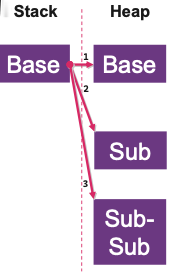
\includegraphics[width=.25\columnwidth]{vererbung}} \\
\hline
\end{tabular}
\subsubsection{Typprüfungen}
\begin{lstlisting}
    //Syntax (Resultat: bool)
    obj is T
\end{lstlisting}
Liefert
\begin{itemize}
    \item true wenn Typ von obj identisch wie T ist
    \item true wenn Typ von obj eine Sub-Klasse von T ist
    \item false wen obj null ist
    \item false wenn Typ von obj eine Basisklasse von T ist
    \item false wenn Typ von obj und T nicht in der gleichen Vererbungshierarchie sind
\end{itemize}
Compilerwarnung wenn erkennbar, dass Ausdruck immer true oder false ist.
\begin{lstlisting}
//Syntax (Resultat: bool)
obj is T

class Base { }
class Sub : Base { } 
class SubSub : Sub { }

public static void Test()
{
    SubSub a = new SubSub();
    if (a is SubSub) { /* ... */ }
        // True
    if (a is Sub) { /* ... */ }
        // True
    if (a is Base) { /* ... */ } 
        // True
    
    a = null;
    if (a is SubSub) { /* ... */ }
        // False / NULL
}
\end{lstlisting}
\subsubsection{Type Casts}
\fat{explizit:}
Compilerfehler wenn
\begin{itemize}
    \item Type Cast nicht zulässig
    \item null in einen Value Type gecastet wird
\end{itemize}
\begin{lstlisting}
class Base { }
class Sub : Base { } 
class SubSub : Sub { }

public static void Test()
{
    Base b = new SubSub();
    Sub s = (Sub)b;
    SubSub ss1 = (SubSub)b;
    SubSub ss2 = (SubSub)null;
    
    // Compilerfehler bei Value Types 
    int i = (int)null;
    // Compilerfehler
    string str1 = (string)s;
    
    // Runtime: InvalidCastException
    object obj = "Hello";
    Base b2 = (Base)obj;
}
\end{lstlisting}
\fat{as-Operator:}
\begin{lstlisting}
//Syntax (Resultat: T)
obj as T
//Compiler übersetzt zu
obj is T ? (T)obj : (T)null
\end{lstlisting}
Anweisung an Compiler, einen Typen in einen anderen umzuwandeln
\begin{lstlisting}
public static void Test()
{
    Base b = new SubSub();
    Sub s = b as Sub;
    SubSub ss1 = b as SubSub;
    SubSub ss2 = null as SubSub;
    
    // Compilerfehler bei Value Types 
    int i = null as int;
    // Compilerfehler
    string str1 = s as string;
    
    // Runtime: null
    object obj = "Hello";
    Base b2 = obj as Base;
}
\end{lstlisting}
\fat{implizit:}
Arbeitet nicht mit Nullable Types
\begin{lstlisting}
//Syntax (Resultat: bool)
//Variable result gecasteten Wert
obj is T result
\end{lstlisting}
\begin{lstlisting}
public static void Test()
{
    Base a = new SubSub();
    if (a is SubSub casted)
    {
        Console.WriteLine(casted);
    }
    
    // Compiler-Output
    SubSub casted = default;    
    if (a is SubSub)
    {
        casted = (SubSub) a;
    }
}
\end{lstlisting}
\subsubsection{Abstrakt \& Versiegelt}
\fat{Abstrakt:}
\begin{itemize}
    \item Kann nicht direkt instanziert werden
    \item Kann beliebig viele Interfaces implementieren
    \item Abgeleitete (nicht abstrakte) Klassen müssen alle abstrakten Members implementieren
    \item Abstrakte Members können nur innerhalb abstrakter Klassen deklariert werden
    \item Dürfen nicht sealed sein
    \item Methoden und Properties sind implizit virtual und dürfen nicht als static oder virtual definiert werden
\end{itemize}
\begin{lstlisting}
abstract class Sequence
{
    public abstract void Add(object x); // Meth. 
    public abstract string Name { get; } // Prop. 
    public abstract object this[int i] // Idx. 
    { get; set; }
    public abstract event EventHandler OnAdd; // Event
    public override string ToString() { return Name; }
}
class List : Sequence
{
    public override void Add(object x)
    { /* ... */ }
    public override string Name
    { get { /* ... */ } }
    public override object this[int i]
    { get { /* ... */ } set { /* ... */ } } 
    public override event EventHandler OnAdd;
}
\end{lstlisting}
\fat{Versiegelt:}
\begin{itemize}
    \item Verhindert das Ableiten einer Klasse
    \item Verhindert versehentliches Erweitern
    \item Methoden können statisch gebunden werden
    \item Members können auch alleine sealed markiert werden, jedoch nur mit override. Kombination mit new und virtual nicht erlaubt
    \item Überdecken von versiegelten Members mit new ist erlaubt, sowie auch virtual
\end{itemize}
\begin{lstlisting}
sealed class Sequence 
{
    public void Add(object x) {}
    public string Name { get{} }
    public object this[int i] { get{} }
    public event EventHandler OnAdd;
}
// Compilerfehler
class List : Sequence { /* ... */ }

abstract class Sequence
{
    public virtual void Add(object x) {}
    public sealed void X() {} // Compilerfehler 
    public virtual string Name { get{} }
    public virtual object this[int i] { get{} } 
    public virtual event EventHandler OnAdd;
}
class List : Sequence
{
    public override sealed void Add(object x) {}
    public override sealed string Name { get {} } 
    public override sealed object this[int i] { get{} }
    public override sealed event EventHandler OnAdd;
}
class MyList : List
{
    public new virtual void Add(object x) {}
    public new virtual string Name { get {} } 
    public new virtual object this[int i] { get{} } 
    public new virtual event EventHandler OnAdd;
}
\end{lstlisting}

\subsection{Methoden}
\subsubsection{Methoden überschreiben}
\begin{lstlisting}
class Base 
{
    public virtual void G() { /* ... */ }
}
class Sub : Base 
{
    public override void G() { /* ... */ }
}
class SubSub : Sub
{
    public override void G() { /* ... */ } 
}
\end{lstlisting}
Subklasse kann Methoden, Properties, Indexer der Basisklasse überschreiben
\begin{itemize}
    \item Basisklasse: virtual um Basis-Methode überschreibbar zu machen
    \item Subklasse: override um Basis-Methode zu überschreiben
\end{itemize}
\fat{Regeln:}
\begin{itemize}
    \item Members sind per Default NICHT virtual und NICHT overrride. Auch nicht, wenn Basis-Member virtual ist
    \item Signatur muss identisch sein, plus gleiche Sichtbarkeit und Rückgabewert
    \item virtual kann nicht mit static, abstract, private oder override kombiniert werden
\end{itemize}
\subsubsection{Dynamic Binding}
Methode des dynamischen Typs wird aufgerufen.
\begin{lstlisting}
Base b = new SubSub();
b.G(); // SubSub.G()
\end{lstlisting}
\fat{Regelwerk:}
\begin{itemize}
    \item Falls Dynamischer Typ (SubSub) konkreter als statischer Typ (Base) und G() virtual ist.
    \item Suche Vererbungs-Hierarchie von oben nach unten nach konkretester Methode G() mit Schlüsselwort override
\end{itemize}
\fat{Methoden überdecken}
Unterbricht Dynamic Binding!
\begin{itemize}
    \item Hinweis für Compiler,dass Member bewusst überdeckt wurde
    \item new kann nicht zusammen mit override verwendet werden
    \item new kann mit virtual verwendet werden
\end{itemize}
\begin{lstlisting}
class Base 
{
    public virtual void H() { /* ... */ }
}
class Sub : Base 
{
    public override void H() { /* ... */ }
}
class SubSub : Sub
{
    //Warnung: entweder override oder überdecken mit new
    public void H() { /* ... */ } 
    //Überdeckt H() von Base/Sub
    public new void H() { /* ... */ } 
    //new nicht verwenden, wenn es keinen Member überdeckt
    public new void I() { /* ... */ }
}
\end{lstlisting}
\fat{Beispiel:}
\begin{lstlisting}
class Base
{
    public virtual void G() { /* ... */ }
    public virtual void J() { /* ... */ }
    public virtual void K() { /* ... */ }
    public virtual void L() { /* ... */ }
}
class Sub : Base
{
    public override void G() { /* ... */ }
    public new void J() { /* ... */ }
    public override void K() { /* ... */ }
    public new virtual void L() { /* ... */ }
}
class SubSub : Sub
{
    public override void G() { /* ... */ }
    public new void J() { /* ... */ }
    public new void K() { /* ... */ }
    public override void L() { /* ... */ }
}

internal class Examples
{
    public static void TestDynamicBinding_J()
    {
        Base b1 = new SubSub();
        b1.J();           // Base.J()
        ((Sub)b1).J();    // Sub.J()
        ((SubSub)b1).J(); // SubSub.J()

        Base b2 = new Sub();
        b2.J();           // Base.J()  

        Sub s = new SubSub();
        s.J();            // Sub.J()
    }
    public static void TestDynamicBinding_K()
    {
        Base b1 = new SubSub();
        b1.K();           // Sub.K()
        ((Sub)b1).K();    // Sub.K()
        ((SubSub)b1).K(); // SubSub.K()

        Base b2 = new Sub();
        b2.K();           // Sub.K()  

        Sub s = new SubSub();
        s.K();            // Sub.K()
    }
    public static void TestDynamicBinding_L()
    {
        Base b1 = new SubSub();
        b1.L();           // Base.L()
        ((Sub)b1).L();    // SubSub.L()
        ((SubSub)b1).L(); // SubSub.L()

        Base b2 = new Sub();
        b2.L();           // Base.L()  

        Sub s = new SubSub();
        s.L();            // SubSub.L()
    }
}
\end{lstlisting}

\subsection{Interfaces}
\subsubsection{Implementation und Verwendung}
\fat{Regeln:}
\begin{itemize}
    \item Eine Klasse kann beliebig viele Interfaces implementieren
    \item Alle Interface-Members müssen auf der Klasse vorhanden sein
    \item override ist nicht nötig ausser allfällige Basisklasse definiert gleichen Member
    \item Kombination mit virtual und abstract ist erlaubt
    \item Implementierte Interface-Members müssen public und dürfen nicht static sein
\end{itemize}
\begin{lstlisting}
interface ISequence {
    void Add(object x);
    string Name { get; }
    object this[int i] { get; set; }
    event EventHandler OnAdd;
}
class List : ISequence {
    public void Add(object x) { /* ... */ }
    public string Name { get { /* ... */ } }
    public object this[int i] 
    { get { /* ... */ } set { /* ... */ } }
    public event EventHandler OnAdd;
}

List list1 = new List();
list1.Add("Hello");

ISequence list2 = new List();
list2.Add("Hello");
\end{lstlisting}
\subsubsection{Name Clashes}
Zwei Interfaces können gleiche Members definieren.
\begin{lstlisting}
interface ISequence 
{
    void Add(object x);
    string Name { get; }
    object this[int i] { get; set; }
    event EventHandler OnAdd;
}
interface IShoppingCart
{
    void Add(object x);
}
\end{lstlisting}
\fat{Szenario 1:}
\begin{itemize}
    \item Signatur identisch
    \item Rückgabetyp identisch
    \item Gleiche Logik für beide Members
    \item Methode regulär implementieren
\end{itemize}
\begin{lstlisting}
class ShoppingCart : ISequence, IShoppingCart 
{
    public void Add(object x) { /* ... */ }
    /* weitere Methoden */
}
//Anwendung
ShoppingCart sc = new ShoppingCart();
sc.Add("Hello");
ISequence sc1 = new ShoppingCart();
sc1.Add("Hello");
IShoppingCart sc2 = new ShoppingCart(); 
sc2.Add("Hello");
\end{lstlisting}
\fat{Szenario 2:}
\begin{itemize}
    \item Signatur identisch
    \item Rückgabetyp identisch
    \item Die Logik ist für beide Members unterschiedlich
    \item Methoden explizit implementieren
\end{itemize}
\begin{lstlisting}
class ShoppingCart : ISequence, IShoppingCart
{
    void ISequence.Add(object x) { /* ... */ }
    void IShoppingCart.Add(object x) { /* ... */ }
    /* weitere Methoden */
}
//Anwendung
ShoppingCart sc = new ShoppingCart(); 
sc.Add("Hello"); // Compilerfehler 
ISequence sc1 = new ShoppingCart(); 
sc1.Add("Hello"); // ISequence.Add 
IShoppingCart sc2 = new ShoppingCart(); 
sc2.Add("Hello"); // IShoppingCart.Add
\end{lstlisting}
\fat{Szenario 3:}
\begin{itemize}
    \item Signatur identisch
    \item Rückgabetyp identisch
    \item Die Logik ist für beide Members unterschiedlich
    \item Default-Verhalten identifizierbar
    \item Methoden regulär \& explizit implementieren
\end{itemize}
\begin{lstlisting}
class ShoppingCart : ISequence, IShoppingCart {
    public void Add(object x) { /* ... */ }
    void IShoppingCart.Add(object x) { /* ... */ }
    /* weitere Methoden */
}
ShoppingCart sc = new ShoppingCart(); 
sc.Add("Hello"); // Add
ISequence sc1 = new ShoppingCart(); 
sc1.Add("Hello"); // Add
IShoppingCart sc2 = new ShoppingCart(); 
sc2.Add("Hello"); // IShoppingCart.Add
\end{lstlisting}
\fat{Szenario 4:}
\begin{itemize}
    \item Signatur identisch
    \item Rückgabetypen verschieden
    \item Die Logik ist für beide Members unterschiedlich
    \item Default-Verhalten identifizierbar
    \item Methoden regulär \& explizit implementieren
\end{itemize}
\begin{lstlisting}
class ShoppingCart : ISequence, IShoppingCart {
    public void Add(object x) { /* ... */ }
    void ISequence.Add(object x) { /* ... */ } 
    int IShoppingCart.Add(object x) { /* ... */ } 
    /* weitere Methoden */
}
ShoppingCart sc = new ShoppingCart(); 
sc.Add("Hello"); // Add
ISequence sc1 = new ShoppingCart(); 
sc1.Add("Hello"); // ISequence.Add 
IShoppingCart sc2 = new ShoppingCart(); 
sc2.Add("Hello"); // IShoppingCart.Add
\end{lstlisting}

\end{multicols*}